% !TEX root = ../main.tex
\chapter{Introduction}

\section{Natural products from \textit{Streptomyces}} % (fold)
\label{sec:natural_products_from_it}

% section natural_products_from_it (end)

\section{Hydrophilic Antibiotics} % (fold)
\label{sec:hydrophilic_antibiotics}

A common molecular parameter to determine hydrophilicity is $\log P$, the logarithm of the partition coefficent between 1-octanol and water\autocite{Leo1971}.
Since accurate solubility prediction is of great importance in drug design, numerous methods have been implemented to calculate $\log P$ from chemical structures.\autocite{Eros2002,VandeWaterbeemd1996,Mannhold2009}

The StreptomeDB~2.0 database provides a unique, manually curated overview of natural products synthesized by \emph{Streptomyces} species.\autocite{Klementz2016}
It contains over 4000 unique compounds produced by over 2500 host organisms and can be utilized to generate an overview of the hydrophilicity of published secondary metabolites.
The distribution of $\log P$ in the dataset (see Figure~\ref{fig:logp_dist}) reveals, that the vast majority ($\sim 75\%$) of structures is on the hydrophobic side of the spectrum.
In reality, the proportion is likely even higher as $\log P$ only applies to uncharged structures, whereas many natural products are ionized under physiological conditions.
The discovery process of \emph{Streptomyces} secondary metabolites seems to favour hydrophobic molecules.
Extraction with organic solvents followed by separation via High-Performance Liquid Chromatography (HPLC) is often used in isolation processes, while techniques more suitable to hydrophilic compounds still need to achieve the same level of prevalence.\autocite{Sticher2008}

\begin{figure}[htbp]
	\centering
	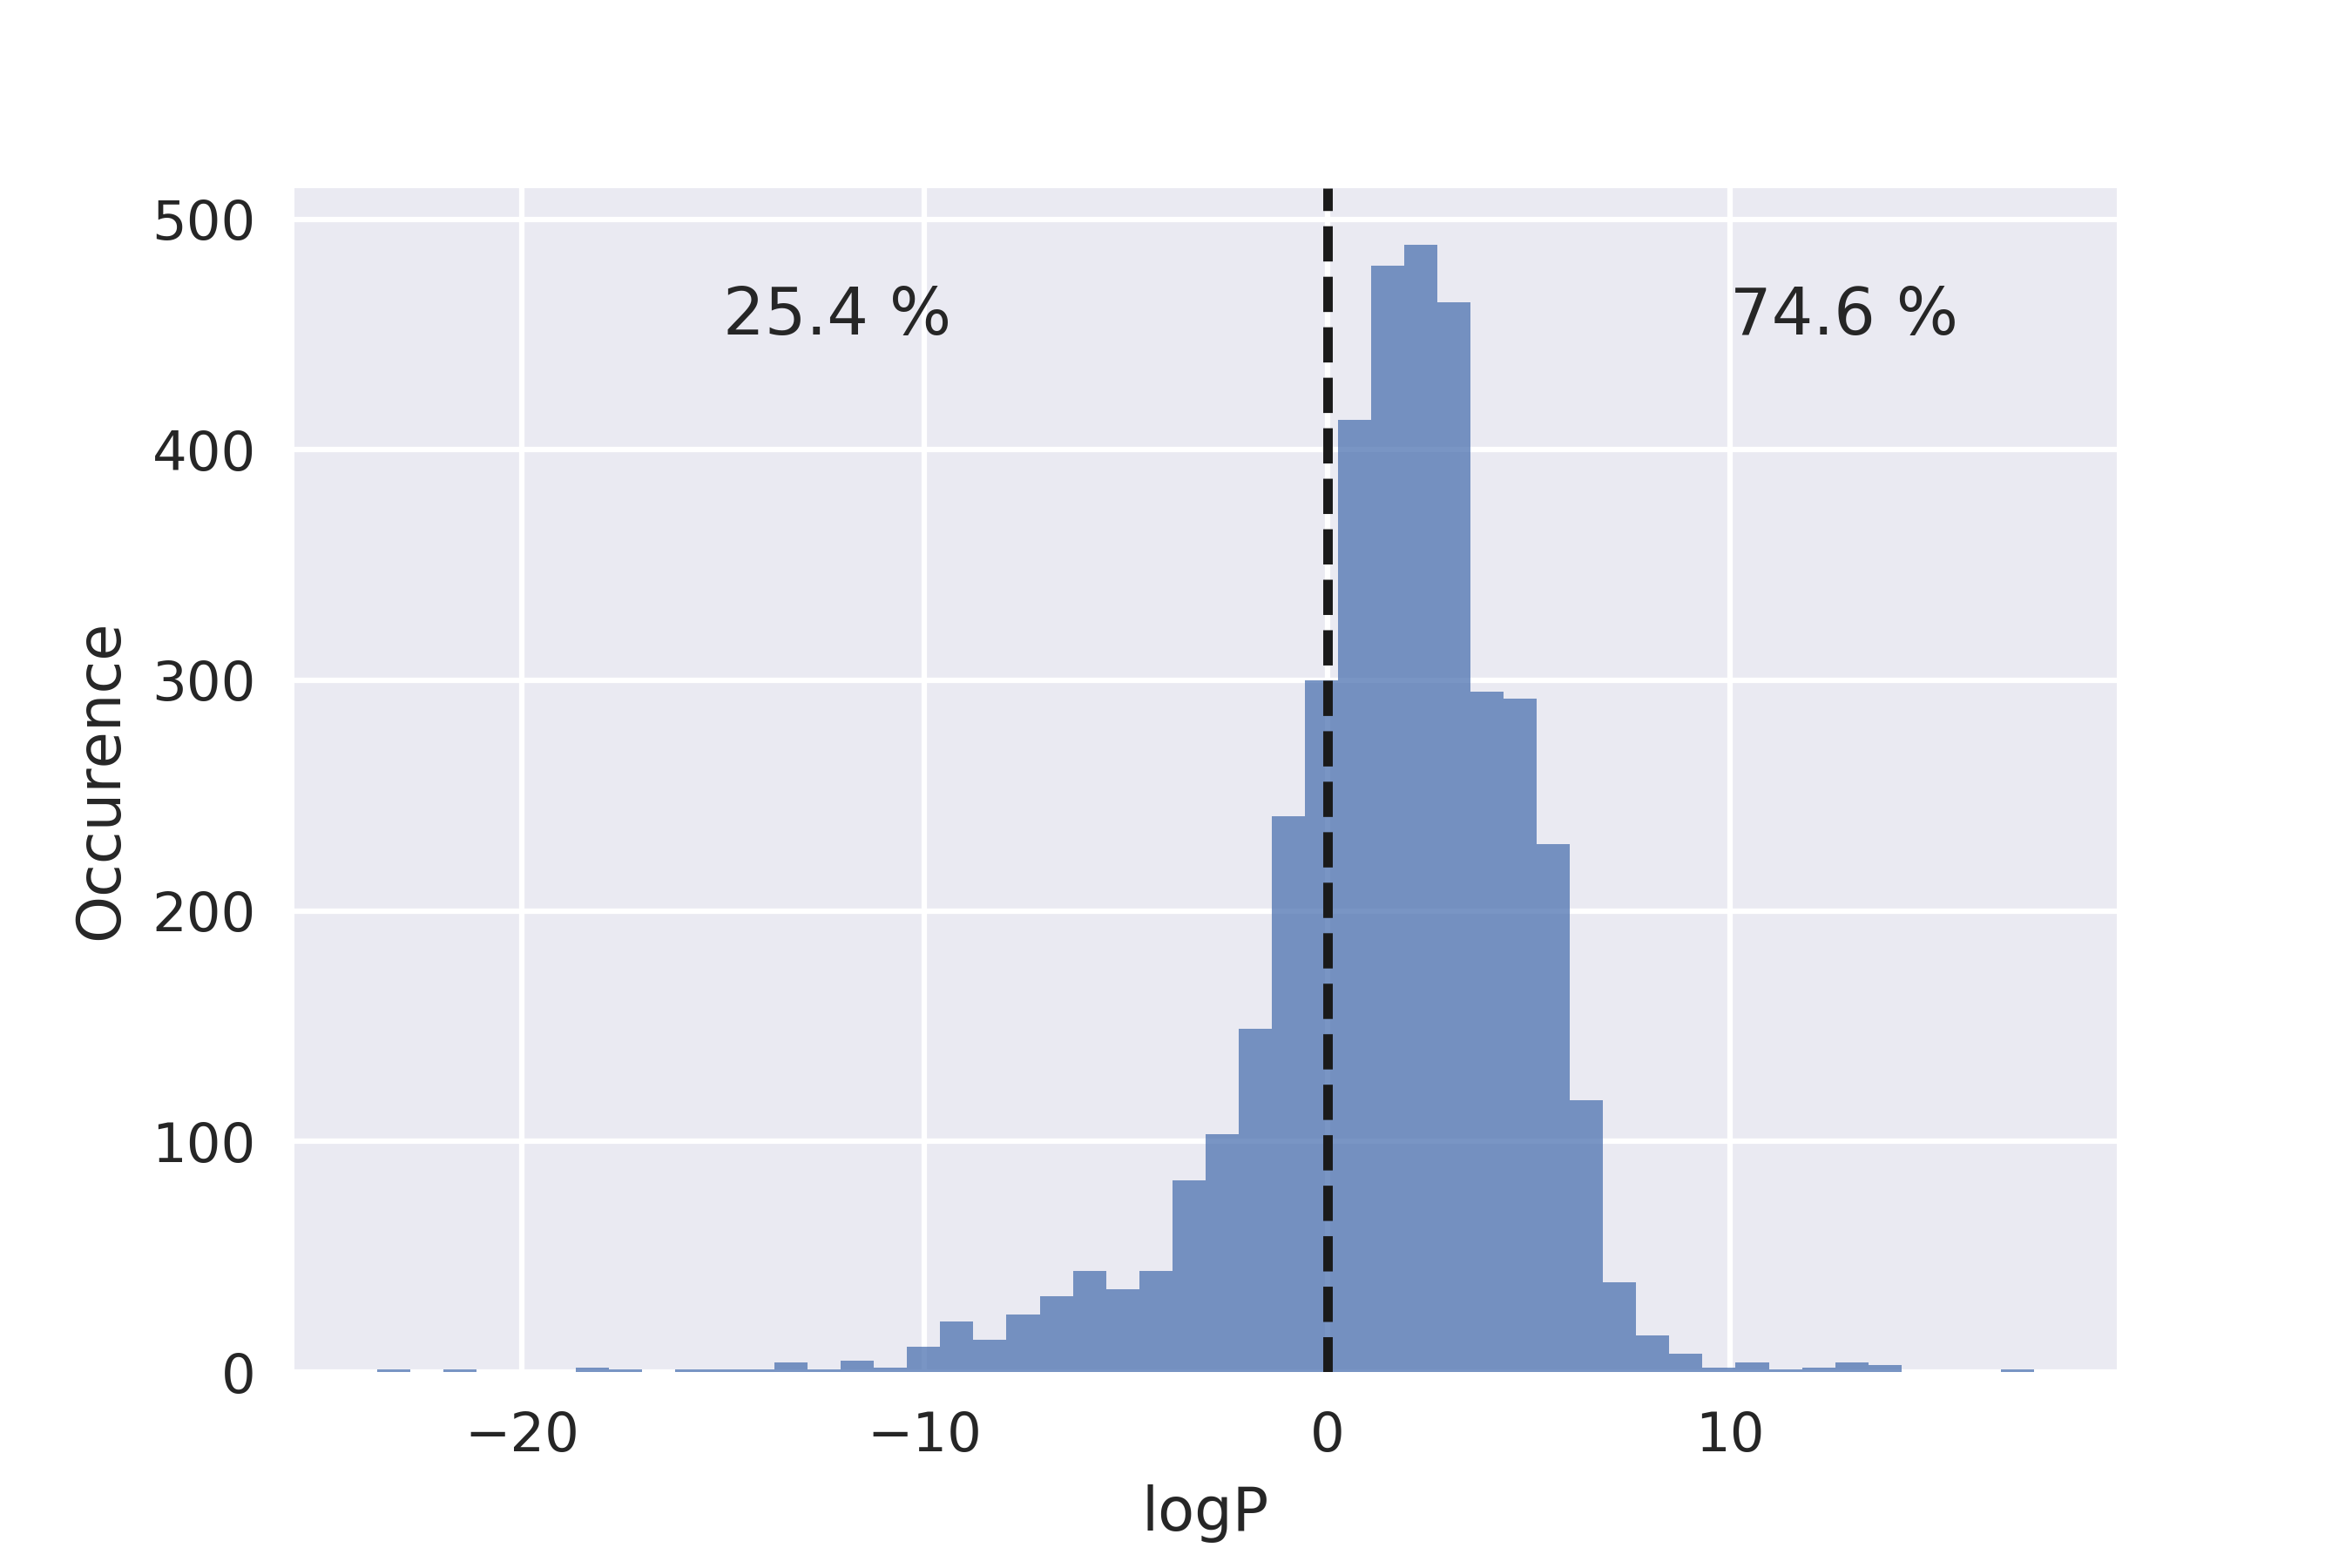
\includegraphics[width=0.7\textwidth]{dist.png}
	\caption[Distribution of logP in the StreptomeDB Database]{%
		\textbf{Distribution of logP in the StreptomeDB Database}
		The molecular partition coefficient (logP) was calculated for 3985 entries in the StreptomeDB 2.0 secondary metabolite database\autocite{Klementz2016} using the descriptor methods implemented in the RDKit cheminformatics suite\autocite{Wildman1999}.
		74.6~\%  of compounds are predicted to have logP value above zero and 25.6~\% equal zero or below.
	}
	\label{fig:logp_dist}
\end{figure}



% section hydrophilic_antibiotics (end)

\section{Antibiotics against Gram-negative bacteria} % (fold)
\label{sec:antibiotics_against_gram_negative_bacteria}

% section antibiotics_against_gram_negative_bacteria (end)

\section{Isolation strategies for hydrophilic natural products} % (fold)
\label{sec:isolation_strategies_for_hydrophilic_natural_products}

% section isolation_strategies_for_hydrophilic_natural_products (end)

\section{Aim of this thesis} % (fold)
\label{sec:aim_of_this_thesis}

% section aim_of_this_thesis (end)
